\afterpage{
    \begin{figure}[t!]
        \centering
        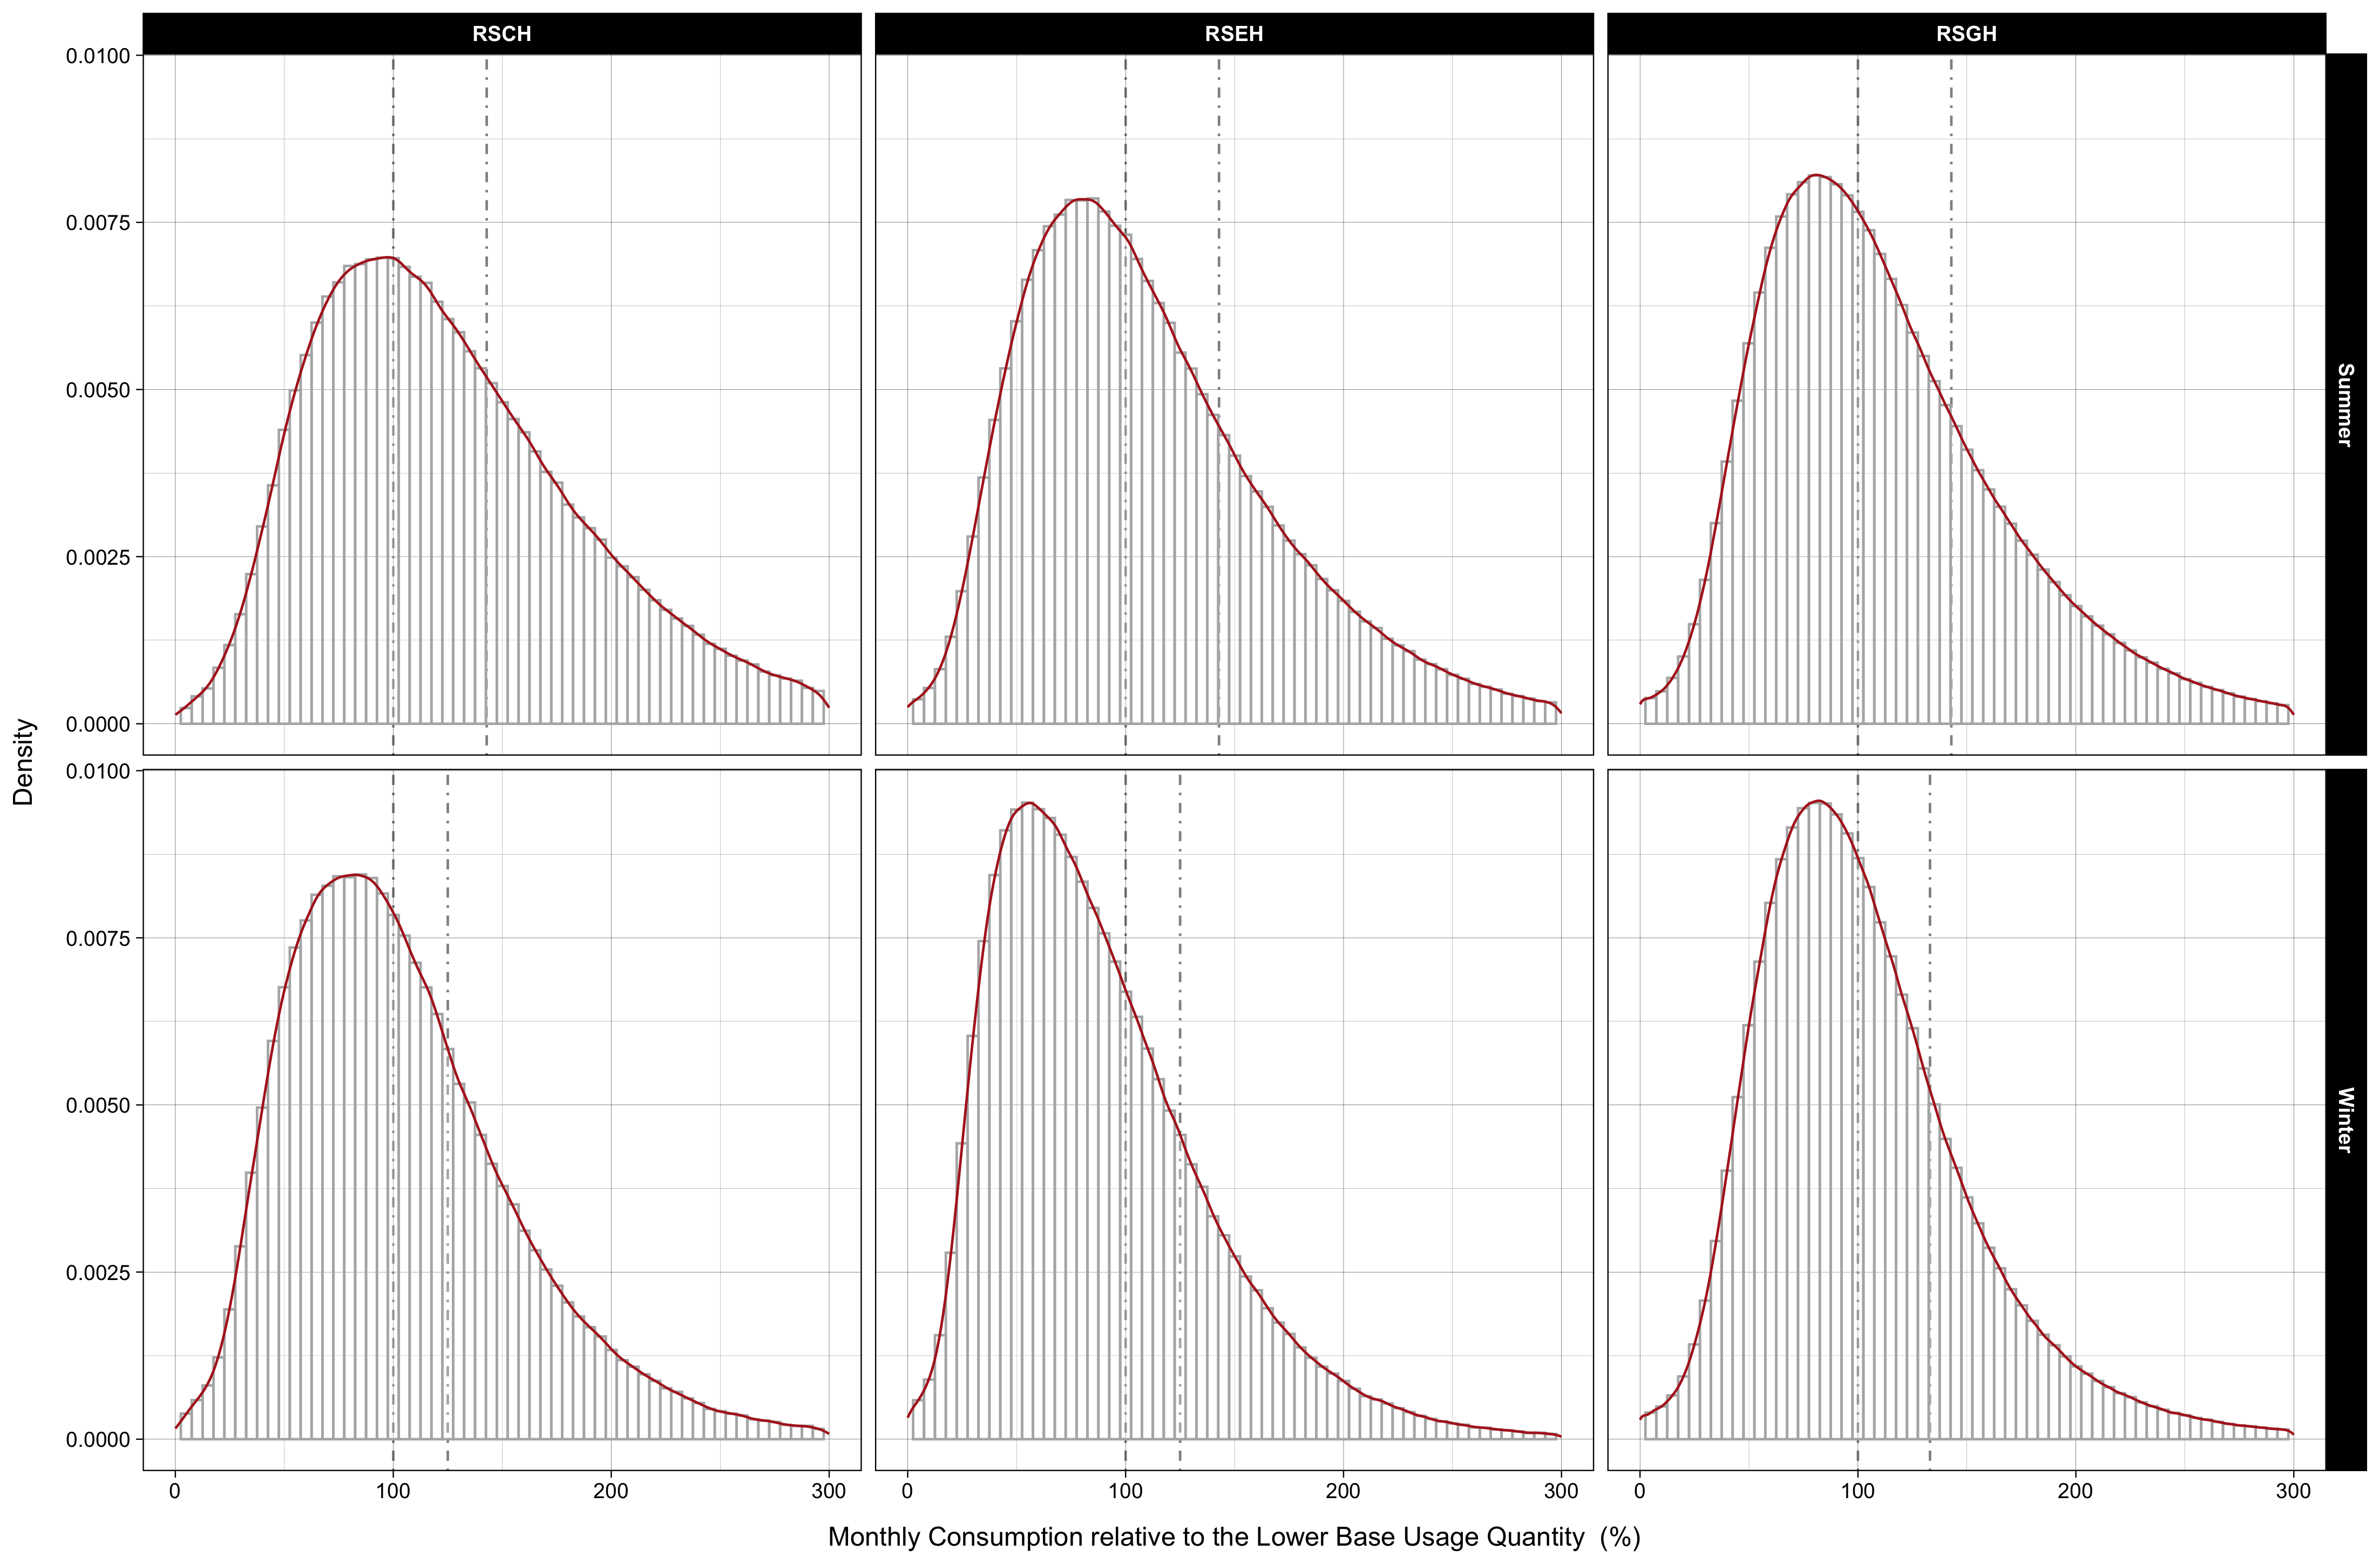
\includegraphics[scale = 0.101]{02_Chapter-1/00A_Figures/Figure_Distribution-of-Electricity-Consumption.png}
        \caption{Distribution of Electricity Consumption by SMUD Residential Customers}
        \caption*{
            {\small
            \textit{Note}: 
            This figure presents histograms, with kernel density estimates, for electricity consumption by SMUD residential customers. Each of the six panels in the figure is for a pair of three major residential rates (i.e., RSCH, RSEH, and RSGH) and two seasons (i.e., summer and winter). Dot-dashed vertical lines in each panel are base usage quantities for the corresponding rate code and season.
        }}
        \label{Figure:SMUD-Billing-Data_Histogram_By-Season-and-Rate-Code}
    \end{figure}
}
Two pieces of evidence support the assumption that base usage quantities do not correspond to jumps in household characteristics. First, as illustrated in Figure \ref{Figure:SMUD-Billing-Data_Histogram_By-Season-and-Rate-Code}, each density plot of the running variable is very smooth, without any bump (i.e., excess mass), around base usage quantities at which marginal prices jump. The set of density plots that show apparent continuity at the thresholds suggests households' inability to precisely adjust their electricity consumption in order not to be subject to a higher marginal price. 

\afterpage{
    \begin{figure}[t!]
        \centering
        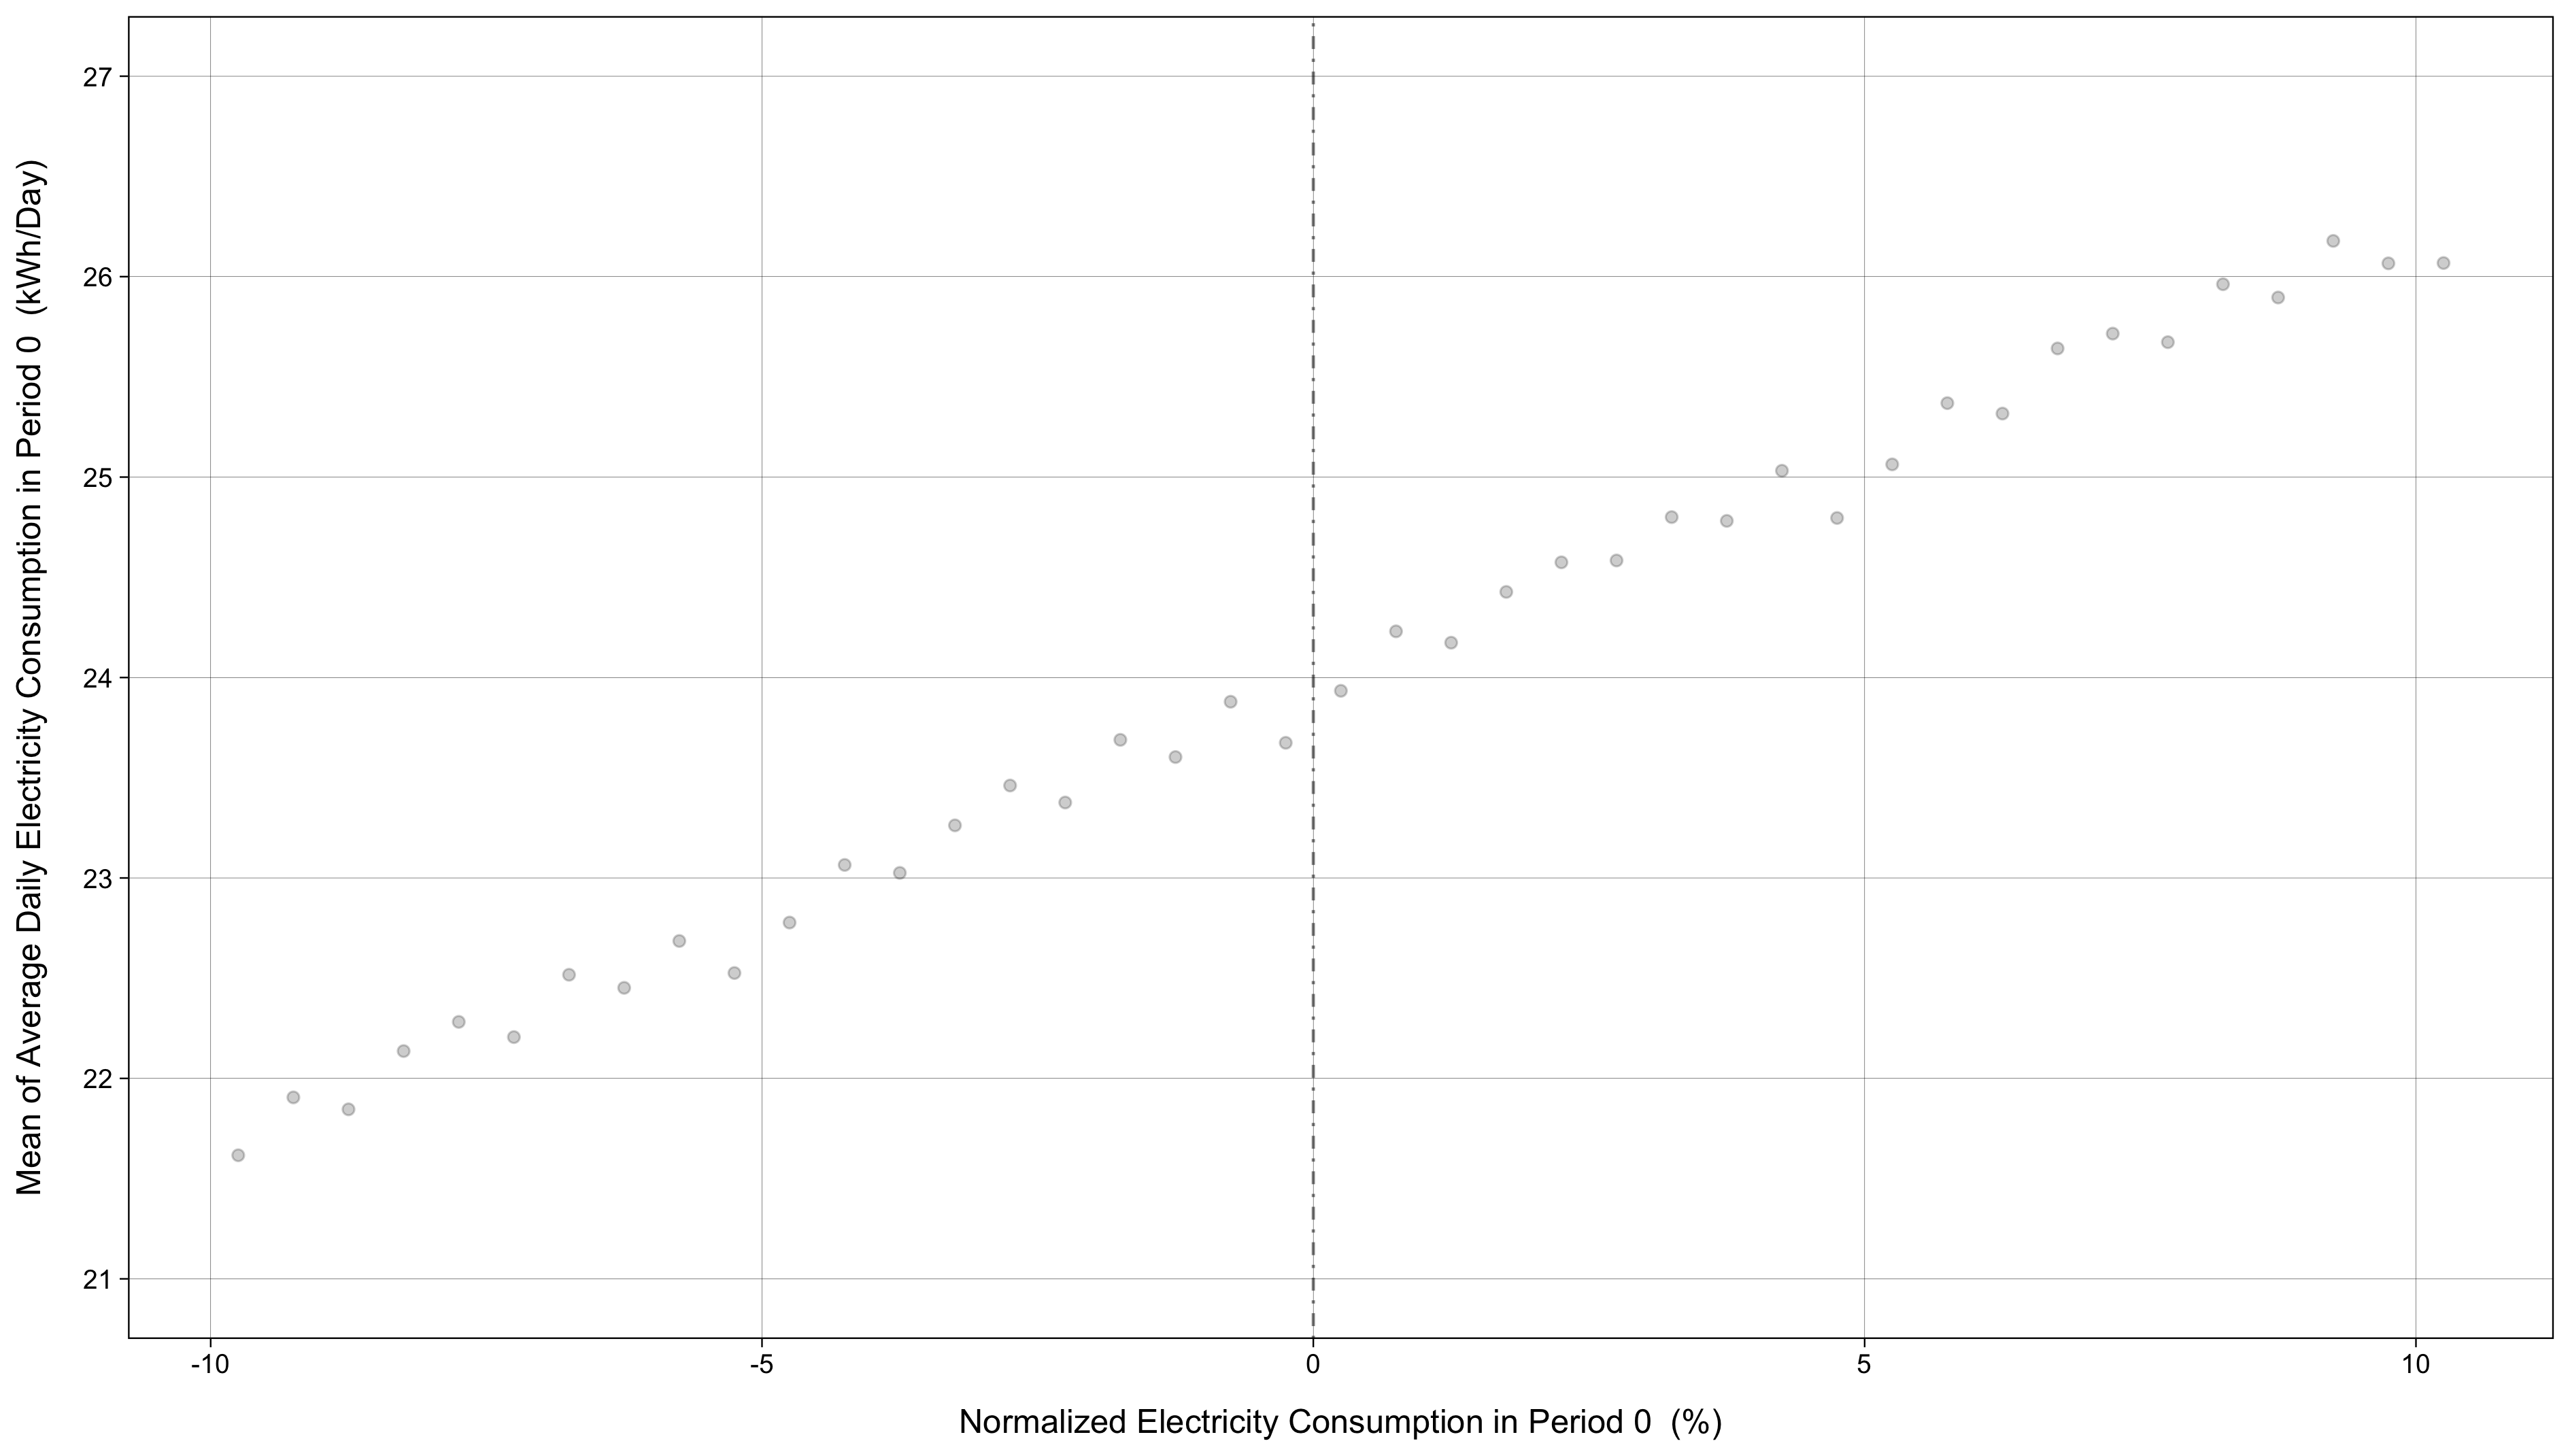
\includegraphics[scale = 0.115]{02_Chapter-1/00A_Figures/Figure_Average-Daily-Electricity-Consumption-in-Period-0-over-NC0.png}
        \caption{Mean of Average Daily Electricity Consumption in Period 0 over $\overline{NC}_{0}$}
        \caption*{
            {\small
            \textit{Note}: 
            In this figure, the scatter points correspond to the average daily electricity consumption in Period 0, calculated by binds with a bandwidth of 1\% of $\overline{NC}_{0}$. As can be seen, the average daily electricity consumption evolves smoothly around the cutoff point (i.e., $\overline{NC}_{0} = 0$). 
        }}
        \label{Figure:Average-Daily-Electricity-Consumption-in-Period-0-over-NC0}
    \end{figure}
}
Second, Figure \ref{Figure:Average-Daily-Electricity-Consumption-in-Period-0-over-NC0} demonstrates that households' average daily electricity consumption during Period 0 evolved smoothly around the lower cutoff point. This figure allows me, at a minimum, not to reject the assumption of local randomization around the base usage quantity, even though examining an observed covariate around the thresholds is not also a direct test for the validity of the assumption.
